\documentclass[oneside,11pt,letter]{article}
% General include (DO NOT MODIFY)
\usepackage{amsmath,graphicx,cite,latexsym,color, amssymb,ifthen,verbatim}

\usepackage{listings, url}
\definecolor{mygreen}{rgb}{0,0.6,0}
\definecolor{mygray}{rgb}{0.5,0.5,0.5}
\definecolor{mymauve}{rgb}{0.58,0,0.82}

\lstset{ %
  backgroundcolor=\color{white},   % choose the background color
  basicstyle=\footnotesize,        % size of fonts used for the code
  breaklines=true,                 % automatic line breaking only at whitespace
  captionpos=b,                    % sets the caption-position to bottom
  commentstyle=\color{mygreen},    % comment style
  escapeinside={\%*}{*)},          % if you want to add LaTeX within your code
  keywordstyle=\color{blue},       % keyword style
  stringstyle=\color{mymauve},     % string literal style
}
\lstset{basicstyle=\small\ttfamily,breaklines=true}

%--------------- Various Style Declarations ----------------------------
\textheight 9in
\topmargin 0in
\headheight 0in
\headsep 0in
\textwidth 6.5in
\oddsidemargin 0in
\evensidemargin 0in
\footskip 0.2in
\parskip 5pt
\parindent 0pt
\topsep 2pt
\partopsep 0pt
\itemsep 0pt
\pagenumbering{arabic}

\definecolor{shade}{gray}{0.85}


\newcommand{\solpagesize}%
{\ifthenelse{\equal{\type}{solutions}}{
\textheight9in
\textwidth6.5in
\oddsidemargin0in
\evensidemargin0in
\topmargin-0.75in
\topskip0in
\footskip0.70in
\pagestyle{empty}
\parskip 5pt
\parindent 0pt
}{}}

\newcommand{\bookletskip}[1] %
{\ifthenelse{\equal{\type}{booklet}}{\vspace{#1 in}}
}

\newcommand{\bookletpage} %
{\ifthenelse{\equal{\type}{booklet}}{\newpage}{}
}

\newcommand{\inbooklet}[1]{\ifthenelse{\equal{\type}{booklet}}{{#1}}}


%%%%%%%%%%%%%%%%%%%%%%%%%%%%%%%%%%%%%%%
% Here are the new definitions of the commands \problem (for main
% text of problem), \problempart (for parts (a), (b) etc of the problem
% and \solution (for text of the solution).  The usage is as follows.
%
%    \begin{enumerate}
%    \problem{label}{main text of first problem}
%    \begin{enumerate}
%    \problempart{text of part(a) of first problem}
%
%    \solution{text of solution to part(a)}
%    \problempart{\text of part(b)}
%
%    \solution{text of solution to part (b)}
%
% ..... and so on for succeeding parts
%
%    \end{enumerate}
%
%    \problem{label}{main text of second problem}
%    \begin{enumerate}
%    \problempart{text of part(a)}
%
%    \solution{text of solution to part(a)}
%    \problempart{\text of part(b)}
%
%    \solution{text of solution to part (b)}
%    \end{enumerate}
%    ........ and so on for other problems
%    \end{enumerate}
%
% Please note that there needs to be a blank line separating
% a problempart command and the succeeding solution command;
% else the problem part and the solution are typeset as one
% paragraph when we are printing both the problem and its
% solution.  However, it is OK if a problempart follows a
% previous solution without an intervening blank line.  Some day I will
% waste some time figuring out a way around this problem

\newcommand{\problem}[2]%
{\item\label{#1}%
\ifthenelse{\(\equal{\type}{problems}\)\or\(\equal{\type}{both}\)}%
 {{\bf[#1]\\}#2}{{\bf[#1]}}}
 % The problem name always prints on the first line (in boldface
 % and inside square brackets.  The problem text prints on
 % succeeding lines if we are printing problems only, or problems
 % and solutions both

  \newcommand{\problempart}[1]%
{\item{\ifthenelse{\(\equal{\type}{problems}\)\or\(\equal{\type}{both}\)}%
 {#1}{}}}
 % The tag ((a), or (b) or (c) etc.) of the text of the part of the problem
 % prints in the margin, and is followed by the text of the problem beginning
 % on the same line if we are printing problems only or problems and
 % solutions both

 \newcommand{\solution}[1]%
{\ifthenelse{\equal{\type}{both}}{{\bf{Solution:\ }}{#1}}%
 {\ifthenelse{\(\equal{\type}{solutions}\)}%
 {#1}{}}}
 % This command does not generate a tag ((a), or (b) or (c) etc.)
 % for the text, but uses the tag generated by the previous 
 % problempart or examproblempart command.  If only the solutions 
 % are being printed, then the text
 % of the solution is printed beginning on the same line as the tag.
 % If both problems and solutions are being printed, then "Solution:"
 % is printed in boldface followed by the text of the solution.

  %%%%%%%%%%%%%%%%%%%%%%%%%%%%%%%%%%%%%%%%%
  
  
 \newcommand{\examproblem}[2]%
{\item {\ifthenelse{\equal{\type}{solutions}}{}{{\bf [#1 points]} #2}}}
% The first argument is an integer specifying the number of points.  The
% first argument (followed by the word "points") is printed inside square
% brackets in boldface.  The second argument is the text of the problem
% itself.


\newcommand{\examproblempart}[1]%
{\item{\ifthenelse{\(\equal{\type}{problems}\)\or\(\equal{\type}{both}\)\or\(\equal{\type}{booklet}\)}%
 {#1}{}}}
 % The tag ((a), or (b) or (c) etc.) of the text of the part of the problem
 % prints in the margin, and is followed by the text of the problem beginning
 % on the same line if we are printing problems only or problems and
 % solutions both

%%%%%%%  ENTER SOME PROBLEM SET SPECIFIC STUFF HERE  %%%%



%%%%%%%%%%%%%%%%%%%%%%
%CHANGE
%.   to booklet to print the problems only
%
%    to both to print problems and solutions
%%%%%%%%%%%%%%%%%%%%%%

\newcommand{\type}{booklet}
%\newcommand{\type}{both}

% Custom adjustments (CHANGE THIS FILE FOR ADDITIONAL ADJUSTMENTS)
\usepackage{tikz}
\newcommand{\cN}{{\cal N}}

\DeclareMathOperator*{\argmin}{\arg\!\min}
\newcommand{\norm}[1]{\left\lVert#1\right\rVert}

%************************************************************************
%                                                                       *
%            End of preamble and beginning of text.                     *
%                                                                       *
%************************************************************************

\begin{document}
%------------------------- Title Page ----------------------------------
\thispagestyle{empty}
\baselineskip2.5ex
{\bf University of Illinois}
\hfill
Spring 2018

{\Large
\begin{center}
{\sf CS\,446: Machine Learning}\\ Homework 5\\
\end{center}
}
{\large
\begin{center}
{\color{red}Due on Tuesday, February 20, 2018, 11:59 a.m. Central Time}
\end{center}
}

\ifthenelse{\equal{\type}{booklet}}{}{}

\ifthenelse{\equal{\type}{booklet}}{
	% !TEX root = HW5.tex
\newcommand{\studSolAA}{
	%%%%%%%%%%%%%%%%%%%%%%%%%%%%%%%%%%%%
	%%
	%%.   YOUR SOLUTION FOR PROBLEM A BELOW THIS COMMENT
	%%
	%%%%%%%%%%%%%%%%%%%%%%%%%%%%%%%%%%%%
	\\For multiclass classification: ii. Labels: each of the different species that can be recognized.\\
	For binary classification: iii. Labels: approved or not-approved.
}

\newcommand{\studSolAB}{
	%%%%%%%%%%%%%%%%%%%%%%%%%%%%%%%%%%%%
	%%
	%%.   YOUR SOLUTION FOR PROBLEM A BELOW THIS COMMENT
	%%
	%%%%%%%%%%%%%%%%%%%%%%%%%%%%%%%%%%%%
	\\For 1-vs-all: $n - 1$ classifiers.\\
	For 1-vs-1: 
	\[
		\frac{n\left(n-1\right)}
		{2}
	\]
}

\newcommand{\studSolAC}{
	%%%%%%%%%%%%%%%%%%%%%%%%%%%%%%%%%%%%
	%%
	%%.   YOUR SOLUTION FOR PROBLEM A BELOW THIS COMMENT
	%%
	%%%%%%%%%%%%%%%%%%%%%%%%%%%%%%%%%%%%
	Let $c_{i, j}$ be the classifier for classes $i$ and $j$, $i, j = 0, 1, ..., K - 1, i < j$. Note that we only have one training example for each class so every example will be in the margin boundary for every $c_{i, j}$.  Below there is a plot of one of these classifiers ignoring all the dimensions that have zero for both points. The marked points are the support vectors and the green line is the decision boundary. It is easy to see that $w$ for this classifier is $(-1, 1)$ (to a scale). \\
	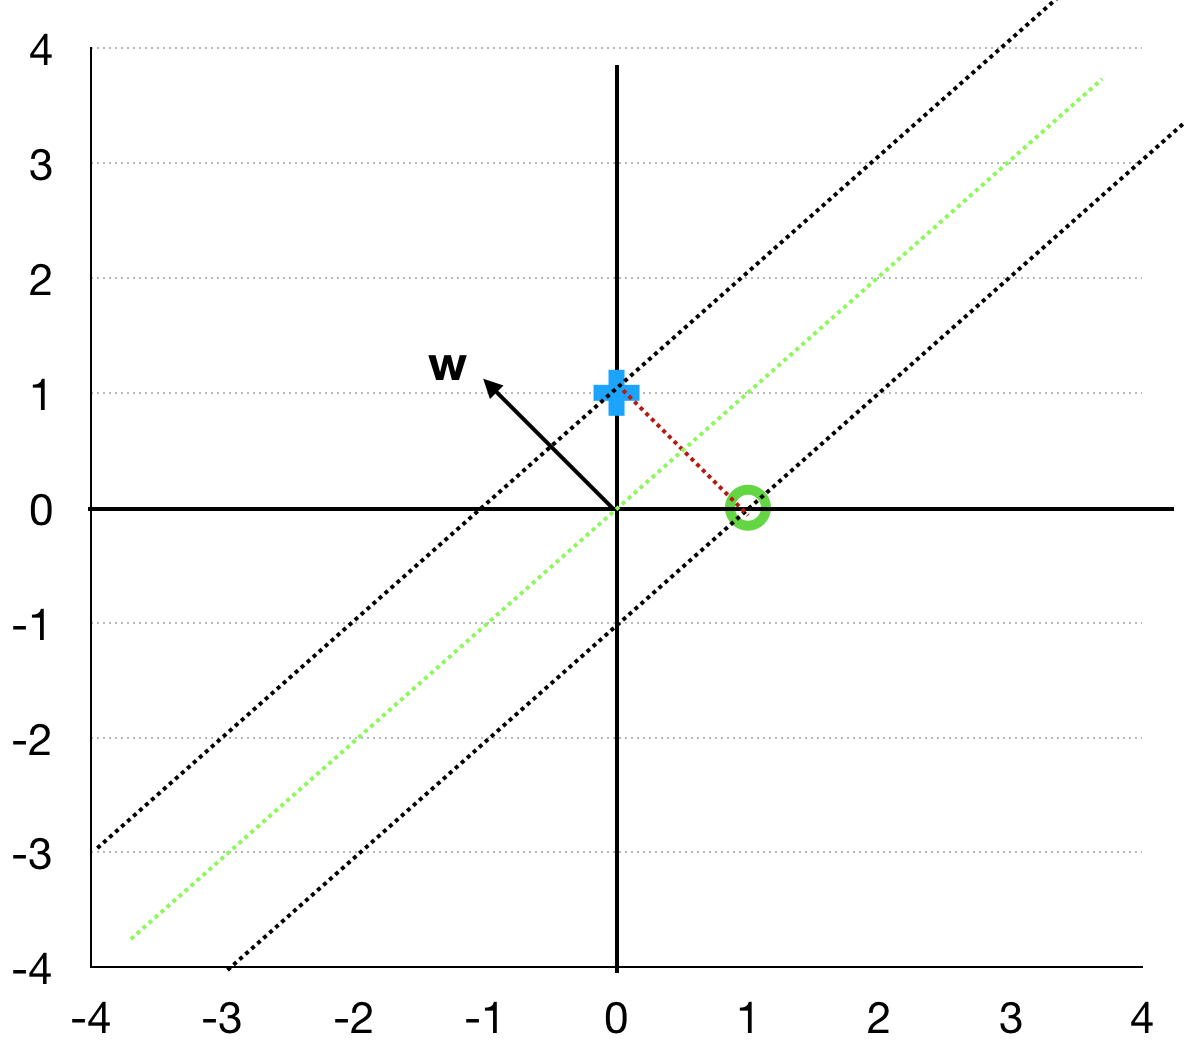
\includegraphics[scale=0.4]{svm.png}
	
	Now consider a test example $x = (x_1, x_2, ..., x_n)$; when tested against $c_{i, j}$ we only care about the components $i, j$ of $x$. In particular, if $x_i > x_j$ then $x$ will be classified as class $i$.\\
	
	Since in particular case is symmetric, e.g. we can take any permutation of the classes and the problem won't change, without loss of generality lets assume that 
	\[x_1 \ge x_2 \ge ... \ge x_n\]
	Note that we can actually assume strict inequality since we are ignoring points in decision boundaries. So,
	\[ x_1 > x_2 > ... > x_n \]
	
	This means that $c_{1, 2}, c_{1, 3}, ..., c_{1, n}$ will all vote for class 1. So \textit{at least} $n-1$ classifiers will vote for class 1. Now note that $c_{2, 3}, c_{2, 4}, ..., c_{2, n}$ will all vote for class 2 so there are at least $n-2$ votes for class 2. By doing this for all $i$ in $c_{i, j}$ we can see that there are exactly $n-i$ classifiers that will vote for class $i$. Therefore, there are \textbf{no} regions in the Euclidean space that will receive the same number of majority votes for more than one class other than the decision boundaries.
}

\newcommand{\constraint}[1]{w_{y^{(#1)}} \phi\left(x^{(#1)}\right) - w_{\hat{y}} \phi\left(x^{(#1)}\right)}
\newcommand{\studSolBA}{
	
	%%%%%%%%%%%%%%%%%%%%%%%%%%%%%%%%%%%%
	%%
	%%.   YOUR SOLUTION FOR PROBLEM A BELOW THIS COMMENT
	%%
	%%%%%%%%%%%%%%%%%%%%%%%%%%%%%%%%%%%%
	Let $w_1, w_2$ be the weights of the classifier for class 0, $w_3, w_4$ for class 1, and, $w_5, w_6$ for class 2.\\
	
	Let's now rewrite the constraints using the given setup. \\
	For $i = 1, \hat{y} = 1$: \\
	\begin{align*}
		\constraint{1} &= 
			\left( 0w_1 + (-1)w_2 \right) - 
			\left( 0w_3 + (-1)w_4 \right)\\
		&= -w_2 + w_4\\
		& \ge 1 - \xi^{(1)}
	\end{align*}
	
	Similarly, for\\
	\[ i = 1, \hat{y} = 2 \rightarrow -w_2 + w_6 \ge 1 - \xi^{(1)} \]
	\[ i = 2, \hat{y} = 0 \rightarrow w_3 - w_1 \ge 1 - \xi^{(2)} \]
	\[ i = 2, \hat{y} = 2 \rightarrow w_3 - w_5 \ge 1 - \xi^{(2)} \]
	\[ i = 3, \hat{y} = 0 \rightarrow w_6 - w_2 \ge 1 - \xi^{(3)} \]
	\[ i = 3, \hat{y} = 1 \rightarrow w_6 - w_4 \ge 1 - \xi^{(3)} \]
	
	We know that $||w||^2 = w_1^2 + w_2^2 + w_3^2 + w_4^2 + w_5^2 + w_6^2$ so the objective function can be rewritten as 
	\[
		\min_{w_1, ..., w_6, \xi^{(i)} \ge 0} \frac{C}{2}\left(	
			w_1^2 + w_2^2 + w_3^2 + w_4^2 + w_5^2 + w_6^2
		\right) + \sum_{i = 1}^n \xi^{(i)}
	\]
	s.t. the six constraints above.
}

\newcommand{\studSolBB}{
	%%%%%%%%%%%%%%%%%%%%%%%%%%%%%%%%%%%%
	%%
	%%.   YOUR SOLUTION FOR PROBLEM A BELOW THIS COMMENT
	%%
	%%%%%%%%%%%%%%%%%%%%%%%%%%%%%%%%%%%%
	By solving for $\xi^{(i)}$ on each of the constraints and taking the max for each of the $\xi$ we have that the function can be written as
	
	\begin{multline*}
		\min_{w_1, ..., w_6} \frac{C}{2}\left(	
			w_1^2 + w_2^2 + w_3^2 + w_4^2 + w_5^2 + w_6^2
		\right)\\
		+ \max \left( 
				1 + w_2 - w_4,
				1 + w_2 - w_6
			\right)\\
		+ \max \left(
				1 + w_1 - w_3,
				1 + w_5 - w_3
			\right)\\
		+ \max \left(
				1 + w_2 - w_6,
				1 + w_4 - w_6
			\right)\\
	\end{multline*}
}

\newcommand{\studSolBC}{
	%%%%%%%%%%%%%%%%%%%%%%%%%%%%%%%%%%%%
	%%
	%%.   YOUR SOLUTION FOR PROBLEM A BELOW THIS COMMENT
	%%
	%%%%%%%%%%%%%%%%%%%%%%%%%%%%%%%%%%%%
	Note that in 2(b) $\max \left(
				1 + w_1 - w_3,
				1 + w_5 - w_3
			\right)$ does not depend on $w_2$ so its derivative will be zero.\\
	Also note that the partial w.r.t $w_2$ of $\max \left( 
				1 + w_2 - w_4,
				1 + w_2 - w_6
			\right)$ will be 1.\\
	We now need to plug $w_t$ in the 
	\[
		\max \left(
				1 + w_2 - w_6,
				1 + w_4 - w_6
			\right) = 
		\max \left( 1 + 1 - (-1), 1 + 2 - (-1) \right)
	\]
	Since the second term is higher the partial w.r.t. $w_2$ of this term is zero.
	Finally we have that:
	\[
		\frac{\partial F}
		{\partial w_2}	 = 
			Cw_2 + 1 + 0 + 0 = 
			C + 1
	\]
}

\newcommand{\studSolBD}{
	\newcommand{\wyhat}{1 + w_{\hat{y}}^\intercal \phi \left( x \right)}
	%%%%%%%%%%%%%%%%%%%%%%%%%%%%%%%%%%%%
	%%
	%%.   YOUR SOLUTION FOR PROBLEM A BELOW THIS COMMENT
	%%
	%%%%%%%%%%%%%%%%%%%%%%%%%%%%%%%%%%%%
	Lets start by remembering that the Chebyshev norm is given by
	\[
		||\mathbf{z}||_{\infty} =
		\lim_{p \rightarrow \infty} \left( \sum_{i} z_i^p \right)^{\frac{1}{p}} =
		\max_i \left( z_i \right)
	\]
	
	Since $f(z) = \exp(z)$ is a monotone function we have that
	\[
		\max_i(z_i) = 
		\ln \max_i \left( \exp \left( z_i \right) \right)
	\]
	
	Combining these two results it follows that
	\begin{align*}
		\max_{\hat{y}}\left( \wyhat \right) &= \ln \max_{\hat{y}} \left( \exp \left( \wyhat \right) \right)\\
		&= \ln \lim_{p 
			\rightarrow \infty} \left( 
				\sum_{\hat{y}}
					\exp \left( \wyhat \right)^p 
			\right)^{\frac{1}{p}}\\
		&= \lim_{p \rightarrow \infty}
			\ln \left( 
				\sum_{\hat{y}}
					\exp \left( \wyhat \right)^p 
			\right)^{\frac{1}{p}}\\
		&= \lim_{\epsilon \rightarrow 0} 
			\ln \left( 
				\sum_{\hat{y}}
					\exp \left( \wyhat \right)^{\frac{1}{\epsilon}} 
			\right)^\epsilon\\
		&= \lim_{\epsilon \rightarrow 0}
			\epsilon \ln
				\sum_{\hat{y}}
					\exp \left( \wyhat \right)^{\frac{1}{\epsilon}}\\
		&= \lim_{\epsilon \rightarrow 0}
			\epsilon \ln
				\sum_{\hat{y}}
					\exp \frac{1}{\epsilon} \left( \wyhat \right)\\
		&= \lim_{\epsilon \rightarrow 0}
			\epsilon \ln
				\sum_{\hat{y}}
					\exp \left( \frac{\wyhat}{\epsilon} \right) \blacksquare
	\end{align*}
} %The students have to fill this file to print the solution
}{
	\input{multiclass_OurSolution} %This file will not be provided to students since it contains the solution
}

\begin{enumerate}

%%%%%%%%%%%%%%%%%%%%%%%%%%%%%%%%%%%%%%
%%%%%  BEGINNING OF PROBLEMS LIST

\examproblem{6}{Multiclass Classification Basics}

%%%%%%%%%%%%%%%%%%%%%%%%%%%%%%%%%%%%%%
%%%%%  BEGINNING OF SUBPROBLEMS LIST
\begin{enumerate}
	
	\examproblempart{Which of the following is the most suitable application for multiclass classification? Which is the most suitable application for binary classification?
	\begin{enumerate}
		\item Predicting tomorrow's stock price;
		\item Recognizing flower species from photos;
		\item Deciding credit card approval for a bank;
		\item Assigning captions to pictures.	
	\end{enumerate}
	}

	% Solution box
	\framebox[14.7cm][l]{
		\begin{minipage}[b]{14.3cm}
			
			\inbooklet{Your answer: \studSolAA}
			
			\solution{\solAA}
			
		\end{minipage}
		
	}

	\examproblempart{Suppose in an $n$-dimensional Euclidean space where $n\geq 3$, we have $n$ samples $x^{(i)}=e_i$ for $i=1...n$ (which means $x^{(1)}=(1,0,...,0)_n, x^{(2)}=(0,1,...,0)_n, ..., x^{(n)}=(0,0,...,1)_n$), with $x^{(i)}$ having class $i$. What are the numbers of binary SVM classifiers we need to train, to get 1-vs-all and 1-vs-1 multiclass classifiers?}
	
	% Solution box
	\framebox[14.7cm][l]{
		\begin{minipage}[b]{14.3cm}
			
			\inbooklet{Your answer: \studSolAB}
			
			\solution{\solAB}
			
		\end{minipage}
		
	}

	\examproblempart{Suppose we have trained a 1-vs-1 multiclass classifier from binary SVM classifiers on the samples of the previous question. What are the regions in the Euclidean space that will receive the same number of majority votes from more than one classes? You can ignore samples on the decision boundary of any binary SVM.}
	
	% Solution box
	\framebox[14.7cm][l]{
		\begin{minipage}[b]{14.3cm}
			
			\inbooklet{Your answer: \studSolAC}
			
			\solution{\solAC}
			
		\end{minipage}
		
	}
	
	%%%%%%%%%%%% END OF SUBPROBLEMS LIST
	
\end{enumerate}

\bookletpage
\examproblem{8}{Multiclass SVM}

%%%%%%%%%%%%%%%%%%%%%%%%%%%%%%%%%%%%%%
%%%%%  BEGINNING OF SUBPROBLEMS LIST
\begin{enumerate}
	Consider the objective function of multiclass SVM as
	$$\min_{w,\xi^{(i)}\geq 0}\frac{C}{2}\|w\|^2 + \sum_{i=1}^n\xi^{(i)}$$ $$ \text{s.t.} \quad w_{y^{(i)}}\phi(x^{(i)}) - w_{\hat{y}}\phi(x^{(i)}) \geq 1 - \xi^{(i)} \quad\forall i=1...n, \hat{y}=0...K-1,\hat{y}\neq y_i$$
	Let $n=K=3$, $d=2$, $x^{(1)} = (0, -1)$, $x^{(2)} = (1, 0), x^{(3)} = (0, 1), y^{(1)} = 0, y^{(2)} = 1, y^{(3)} = 2$, and $\phi(x)=x$.
	\examproblempart{
		Rewrite the objective function with $w$ being a $Kd$-dimensional vector $(w_1,w_2,w_3,w_4,w_5,w_6)^\top$ and with the specific choices of $x$, $y$ and $\phi$.
	}

	% Solution box
	\framebox[14.7cm][l]{
		\begin{minipage}[b]{14.3cm}
			
			\inbooklet{Your answer: \studSolBA}
			
			\solution{\solBA}
			
		\end{minipage}
		
	}

	\examproblempart{
		Rewrite the objective function you get in (a) such that there are no slack variables $\xi^{(i)}$.
	}

	\framebox[14.7cm][l]{
		\begin{minipage}[b]{14.3cm}
			
			\inbooklet{Your answer: \studSolBB}
			
			\solution{\solBB}
			
		\end{minipage}
		
	}

	\examproblempart{
		Let $w_t=(1,1,1,2,1,-1)^\top$. Compute the derivative of the objective function you get in (b) w.r.t. $w_2$, at $w_t$, where $w_2$ is the weight of second dimension on Class 0 (in case you used non-conventional definition of $w$ in (a)).
	}

	\framebox[14.7cm][l]{
		\begin{minipage}[b]{14.3cm}
			
			\inbooklet{Your answer: \studSolBC}
			
			\solution{\solBC}
			
		\end{minipage}
		
	}
	
	\examproblempart{
		Prove that
		$$\max_{\hat{y}}\left(1+w_{\hat{y}}^\top\phi(x)\right)=\lim_{\epsilon\rightarrow0}\epsilon\ln\sum_{\hat{y}}\exp\left(\frac{1 + w_{\hat{y}}^\top\phi(x)}{\epsilon}\right).$$
	}

	\framebox[14.7cm][l]{
		\begin{minipage}[b]{14.3cm}
			
			\inbooklet{Your answer: \studSolBD}
			
			\solution{\solBD}
			
		\end{minipage}
		
	}

	%%%%%%%%%%%% END OF SUBPROBLEMS LIST

\end{enumerate}	

\end{enumerate}
\end{document}

\grid
\grid
\grid
\grid
